%\subsubsection*{Software Testing 14.11}
%WARUM SOLLTE GETESTET WERDEN´?
%WIESO END2END UND UNIT TEST?
%PROJEKTE SCHREITERN WEGEN MANGELHAFTE TESTING \%
%Einer der Gründe dafür ist, dass das Risiko, gar nicht oder zu wenig zu testen, erkannt wurde.
%Unter anderem, weil es klar/verstanden wurde, wie riskant ist, Testaktivitäten zu überspringen oder nicht genug Testing durchzuführen.
In der Vergangenheit haben Unternehmen das Risiko bei der Entwicklung ihrer Projekte unterschätzt. Die waren dazu gezwungen, ihren Betrieb zu unterbrechen, oder haben aufgrund von Fehlern in ihren Anwendungen Kunden verloren. Ein Beispiel dazu ist \textit{Starbucks}, welches im Jahr 2015 etwa 60\% der Filialen in den USA und Kanada wegen eines Softwarefehlers in seinem Kassensystem schließen musste{\cite{QS1}}. Ein weiterer Fall war \textit{Nissan} im Jahr 2014, als fast 1 Million Fahrzeuge wegen eines Softwarefehlers in den Airbag-Sensoriksystemen zurückziehen musste{\cite{QS2}}. Unter die Vorteile, welche das Software-Testing bietet zählen die Risikoverringerung bei den Softwareprojekten, eine Erhöhung der Softwarequalität, schnelle Fehlerfindung, die Aufgabentrennung zwischen dem Software-Testing und der -entwicklung.  Aus diesem Grund wurden \textit{Unit-} für das Backend und \textit{End-to-End-Tests} für das Frontend geschrieben. 
\\\\
Für das Unit-Testing im Backend wird das Testingframework \textit{Jest} und für das Frontend \textit{Cypress} verwendet. Beide Frameworks stehen an die ersten Plätzen in der Ranking von Test-Frameworks von \textit{OpenBase} veröffentlicht{\cite{QS3}}.

\subsubsection*{Unittest}
Dieser Art von Test dient dazu, die korrekte Funktionsweise einer Codeeinheit zu überprüfen. In den meisten Programmiersprachen ist das eine Funktion, ein Unterprogramm oder eine Methode. %Für dieses Projekt wurde das Jest Framework verwendet. 
Dazu werden die Testkomponenten mit der Funktion \textit{describe} definiert. Innerhalb einer Komponente werden die Testfälle selbst mit \textit{test} oder dem alias \textit{it} definiert. Außerdem lassen sich Funktionen definieren, die nach oder vor jedem oder allen Testfällen ausgeführt werden sollen. Dies ermöglicht atomare Tests, dessen Ergebnisse nicht durch andere Testfälle verfälscht werden und. Die Testqualität wird somit erhöht. Die Datenbankschemata werden mit Hilfe von \textit{mongodb-memory-server} getestet. Dies erlaubt die Erstellung einer nicht-persistenten Datenbank im Speicher. Die Datenbank ist am Anfang leer und wird nach jedem Testfall gesäubert, um die Atomarität zu gewährleisten.
Durch Tests der Datenstruktur wird gewährleistet, dass es keine Abweichungen gibt zwischen den Daten, die erwartet werden und denen, die erhalten werden. Tests der Middlewarefunktionen von Mongoose prüfen, ob komplexere Anwendungen, wie das Hashen des Passworts bei dessen Speicherung wie gewünscht ausgeführt werden.
\\\\
Die Tests der GraphQl-Schnittstelle setzen voraus, dass die Datenbank wie gewünscht funktioniert und die gewünschten Daten liefert und speichert.
In verschiedenen Testfällen werden dazu die entsprechenden Resolver geprüft. Dazu wird mit dem Paket \textit{apollo-server-integration-testing} ein Testclient erstellt, der mit \textit{query-} und \textit{mutation-}Abfragen ähnlich wie der richtige Client abgefragt werden kann. Der Testclient unterstützt keine Express-Middleware, welche im Projekt den Nutzer autorisiert und authentifiziert. Diese Funktion musste daher nachgeahmt werden. 
%Before/after all; damit der Zustand zurücksetzen kann.
%Ein TF darf nur 1 Sache testen. 
%1 Beispiel erläutern (User)
%Screenshot von Ergebnisse
%Beschreibung von Screenshot: 1. Zeile gibt an

\subsubsection*{End-to-End Testfälle}
\textit{Cypress} ist ein Testautomatisierungswerkzeug für End-to-End-Tests und UI-Tests. 
%\\\subsubsection*{Testautomatisierung}
Die Automatisierung von Testfällen maximiert die Effizienz, wenn Testfälle in den Kontinuierliche-Integration(Continuous integration) Workflows einbezieht werden. Neuer Code kann automatisch getestet werden, zum Beispiel jedes Mal, wenn ein neues Push-Request erstellt wird.
\begin{figure}[h!]
	\centering
    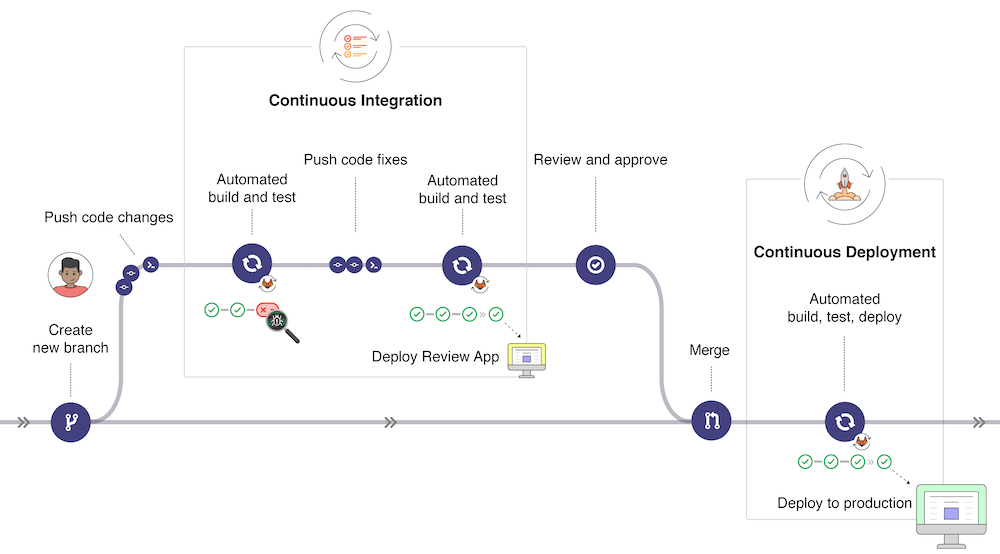
\includegraphics[width=\textwidth]{sources/Gitlab-CI.png}
	\caption{Gitlab-CI/CD Workflow}
	\label{fig:Continuous_integration_workflow} {\cite{GLAB1}}
\end{figure}

%\subsection*{Testing bei diesem Projekt}
Die \autoref{fig:Cy_Test_running} zeigt in der linken Spalte die Schritte eines Tests, die alle erfolgreich durchgeführt wurden und mit grüner Farbe markiert sind. Auf der rechten Seite die Benutzeroberfläche, auf der die Testschritte automatisch ausgeführt werden.
\\
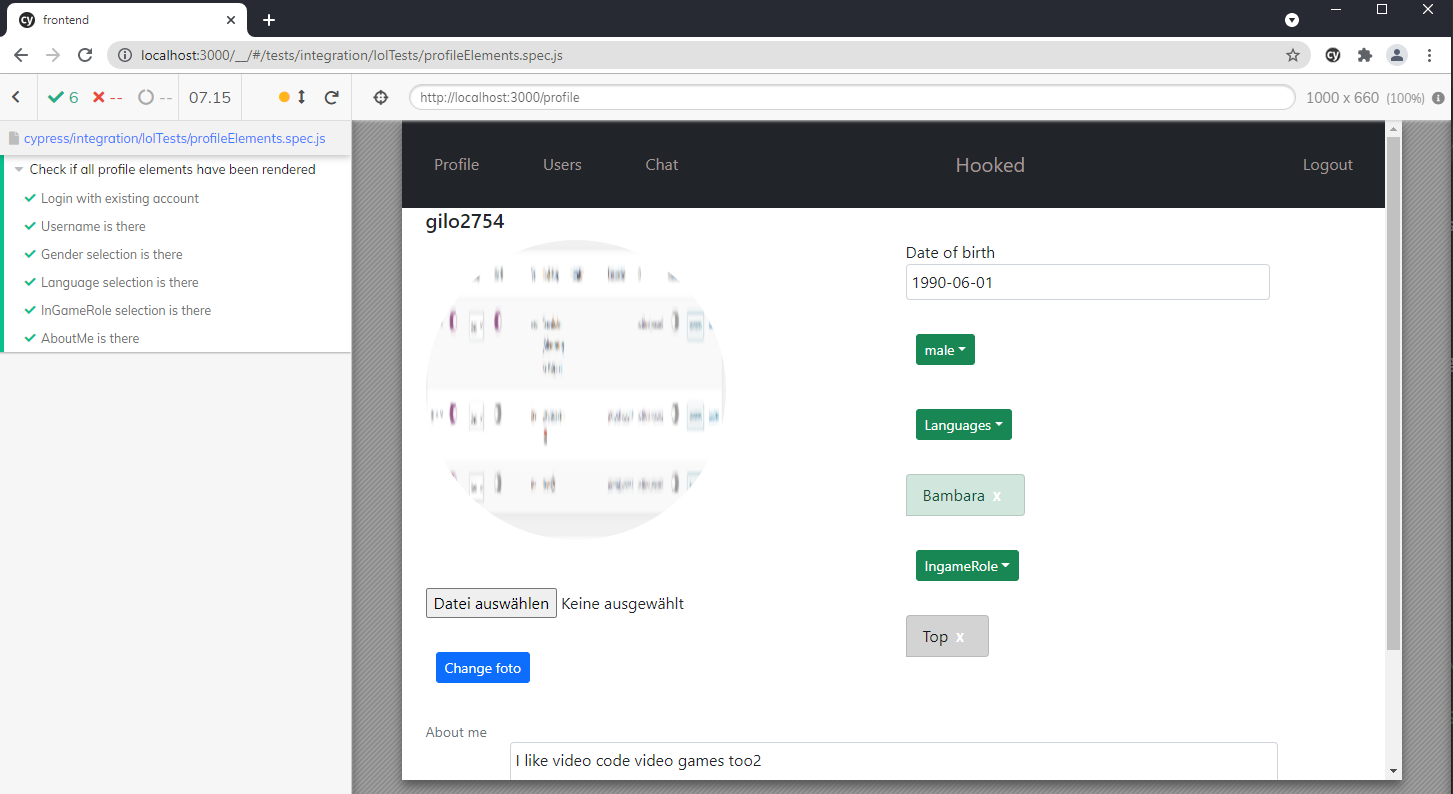
\includegraphics[width=\textwidth]{sources/Cy_Test_running.png}
\begin{figure}[h!]
	\centering
	\caption{Grafische Sicht eines Testlauf bei Cypress. 
	Quelle: eigene Darstellung}
	\label{fig:Cy_Test_running}
\end{figure} 

%Ergebnise der ganzen Testlauf
\begin{comment}
\paragraph{}
%Nachstehend einer Überblick über die Testfälle bei Cypress.\\


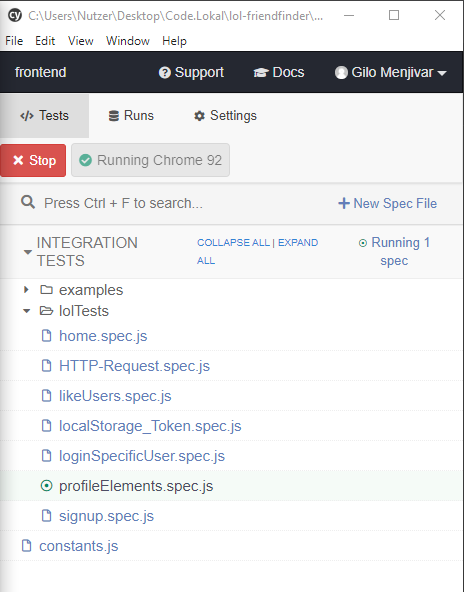
\includegraphics[width=0.5\textwidth]{sources/Cy_Test_Cases.png}
\begin{figure}[ht]
	\centering
	\caption{Testfälle in Cypress. 
	Quelle: eigene Darstellung}
	\label{fig:Cy_Test_Cases}
\end{figure} 

Obwohl das Projekt relativ klein ist, wurde die Wichtigkeit von automatisierten Tests nicht unterschätzt.
\\
Für das Frontend wurden End-to-End Testfälle mit Cypress geschrieben.
Auf diese Weise ist es möglich in Sekundenschnelle festzustellen, ob etwas in unserer Anwendung defekt ist.

Ein Szenario, in dem dies hilfreich ist, ist, wenn eine Unterkomponente in anderen Komponenten verwendet wird.

Durch die Änderung der Unterkomponente kann sich diese in einer unerwünschten Weise verhalten.
\\
Das ist der Fall bei der Komponente AvatarImage.
Dies ist eine Funktionskomponente, die 3 Parameter erhält: Größe des Bildes, Bild-URL und Benutzername.

Zu Beginn des Projekts wurde nicht daran gedacht, die Größe des Bildes über einen Parameter dieser Funktion zu steuern. Im Laufe des Projekts wurde uns klar, dass wir die Logik in diesem Element wiederverwenden konnten.
\\
Innerhalb der Komponente wird geprüft, ob eine URL existiert, und wenn ja, wird das mit dem Link verbundene Bild gezeichnet. Falls es keine URL  angegeben wurde, werden die ersten beiden Buchstaben des Benutzernamens verwendet, um ein Standardsymbol zu erzeugen.

In der aktuellen Version des Codes wird diese Komponente in vier anderen Komponenten wieder verwendet.
Wenn das Projekt weiter wachsen würde, würde auch die Möglichkeit von Fehlern im Code zunehmen. Fehler zu finden, wäre in dem Fall aufwändiger.

Ohne automatisierte Tests, ist manuelles Testing nötig.
\\
Im Anhang 2 befindet sich ein Code-Auszug eines Testfälles End-to-End. 
\end{comment}
%%POSIBLEMENTE ESTE NO ES ELMEJOR EJ PUESTO QUE NO SE ESTA PROBANDO EL TAMANIO LAS IMAGENES EN LAS PRUEBAS DE CYPRESS
%% SIN EMBARGO EL HECHO DE REUTILIZAR LOGICA DE CIERTOS ELEMENTOS ES MUY RELEVANTE Y DEBERIA SER INCLUIDA EN OTRA PARTE %DEL REPORTE
%BUSCAR OTRO EJ. DONDE EL TESTING COBRA MAS RELEVANCIA

